% Template for final reports and dissertations (Instituto Politécnico de Beja)
% Version 0.8.1, 2021/10/01
% Author: João Paulo Barros, joao.barros@ipbeja.pt
% Com contribuições de Henrique Água-Doce, Nuno Mourinho e Raul Carvalho. 


%para texto em Português
\documentclass[PT]{ipbeja-format}
%for text in English
%\documentclass[]{ipbeja-format}



% Para preencher 

\newcommand{\ESCOLA}{Escola Superior de Tecnologia e Gestão}
%\newcommand{\ESCOLA}{Escola Superior de Educação}
%\newcommand{\ESCOLA}{Escola Superior Agrária}
%\newcommand{\ESCOLA}{Escola Superior de Saúde}


\newcommand{\CURSO}{Licenciatura em Engenharia Informática}

\newcommand{\TITULO}{Sistema de apoio à decisão para o turismo no Alentejo}
\newcommand{\SUBTITULO}{Sistema de apoio à decisão com base em \textit{Data Mining} para o turismo no Alentejo}


\newcommand{\NOMEALUNO}{Gonçalo Amaro\\Pedro Tomás\\Vítor Abreu\\}

\newcommand{\LOCAL}{Beja}


 %se for um estágio deve ser retirado o comentário da linha seguinte e indicar o orientador na entidade de acolhimento do estágio
%\newcommand{\ORIENTADORENTIDADE}{Título académico e nome do(a) orientador(a) na entidade de acolhimento, NomeDaEntidade, por exemplo "Eng. Nome Completo ou Abreviado}

\newcommand{\ORIENTADORIPBEJAA}{Doutora Isabel Brito}
% se existir segundo orientador do IPBeja, retirar o comentário da linha seguinte
%\newcommand{\ORIENTADORIPBEJAB}{Colocar o título Académico e nome do(a) segundo(a) docente orientador(a), se existente} 


%Completar e comentar um dos seguintes dois \newcommand
%\newcommand{\DECLARACAOPROJETO}{Relatório de projecto de fim de curso apresentado na\linebreak \ESCOLA{} do Instituto Politécnico de Beja}
\newcommand{\DECLARACAO}{
Relatório de Projecto Final, realizado na cadeira de Projecto Integrado, apresentado na\linebreak \ESCOLA{} do Instituto Politécnico de Beja}

% retirar comentário e preencher se existente
%\newcommand{\DEDICATORIA}{ texto a colocar}

\usepackage[]{hyperref}
\hypersetup{hidelinks,hypertexnames=true}

\begin{document}
\pagenumbering{roman}
\setcounter{page}{1}
\folhacapa % 2.1 das normas
\folharosto % 2.3 das normas
%%%%%%%%%%%%%%%%%%%%%%%%%%%%%%%%%%%%%%%%%%%%
\frontmatter % parte inicial

\clearpage
\chapter{Resumo}
\section*{\textit{\TITULO}\\  {\small{\textit{\SUBTITULO}}}}


\textit
Tendo em vista uma sustentável, duradora e benéfica relação entre o turismo e o património histórico-cultural há que seguir uma estratégia. Existem várias estratégias, porém a tomada na elaboração deste trabalho foi a monitorização de fluxos de visitantes. Esta monitorização pode ser realizada através de um sistema de informação como o TripAdvisor, Zoomato e Booking, que foram os escolhidos na elaboração do trabalho, o armazenamento dos dados, ou seja, o desenvolvimento de uma base de dados em SQL, o processamento de dados usando técnicas para normalizar e analizar textos, assim como a extração das "keywords" e análise de opinião que seriam mais tarde úteis na elaboração de gráficos como medida para uma fácil visualização dos resultados acerca dos resulatos obtidos, indicando muitos aspetos interessantes acerca das preferências turísticas dentro dos patrimónios.

\clearpage
\chapter{Abstract}
\section*{\textit{Decision support system for tourism in Alentejo}\\  {\small{\textit{Decision support system based on Data Mining for tourism in Alentejo}}}}

\textit
In view of a sustainable strategy, historical establishments and cultural establishments between tourism and all places, such as hotels, in addition to historical and cultural establishments, a strategy must be followed. Several strategies, however the elaboration in the elaboration of this workflow was monitoring. This monitoring can be carried out through an information system such as TripAdvisor, Zomato and Booking, which were chosen in the elaboration of the work, the storage of data, that is, a database in SQL, the processing of data using techniques to normalize and study, as well as the extraction of "key words" and opinion analysis that will later be useful in the elaboration of measures for an easy visualization of the results about the obtained results, often interesting about the relevant issues obtained within the heritages.



% Se pretender remover, comente a linha seguinte, caso contrário preencha o ficheiro agradecimentos.tex
\clearpage
\agradecimentos

O relatório de projeto final da cadeira de Projeto Integrado decorre de uma experiência que exigiu trabalho e esforço para alcançarmos os objetivos pretendidos. Como tal, agradecemos a disponibilidade, acompanhamento atento e
colaboração demonstrados pela professora Isabel Brito, agradecemos também o seu apoio, incentivo, confiança e essencialmente por nos ter guiado para uma melhor execução do trabalho.




\clearpage
\indicegeral  
\clearpage
\indicedefiguras % Remover se houver menos de 5 figuras
\clearpage
\indicedetabelas % Remover se houver menos de 5 tabelas
\clearpage
\indicedelistagens % Remover se houver menos de 5 listagens

% No caso de se verificar "um número significativamente elevado de abreviaturas e siglas" deve retirar-se o 
% comentário da linha seguinte e preencher o ficheiro parte-inicial/abreviaturas.tex
%\chapter{Abreviaturas e Siglas}

\begin{longtable}{p{.15\textwidth} p{.85\textwidth}} 

IPBeja & Instituto Politécnico de Beja\\
UML & Unified Modelling Language\\
... & ...

\end{longtable}
 

%%%%%%%%%%%%%%%%%%%%%%%%%%%%%%%%%%%%%%%%%%%%
\mainmatter  \pagestyle{ruled} % parte principal
\pagenumbering{arabic}

\chapter{Introdução}
\label{intro}

% deve substituir as duas linhas seguintes pelo texto da introdução

\section{Objectivo do trabalho}
Este trabalho tem como principal objectivo a monitorização de fluxos de visitantes para identificar boas práticas, tendo sempre foco na criação de uma benéfica, sustentável e duradoura relação entre o turismo e o património. Para essa monitorização ser realizada, será necessário desenvolver um sistema de informação que recolha, armazena, processa e comunica dados e informação sobre as visitas ao património dos turistas nacionais e estrangeiros. Para que a essa monitorização seja realizada devidamente, será necessário que sejam realizadas algumas etapas, das quais seriam:

\begin{enumerate}
    \item A recolha de dados sobre as visitas dos turistas nacionais e estrangeiros ao património cultural de Beja, destacando-se dessa mesma recolha, as atracções, hotéis e restaurantes, e tendo como origens as fontes,  \textit{"TripAdvisor"}, \textit{"Booking"}, \textit{"Zomato"}. Para que a recolha de dados fosse realizada das devidas fontes foi necessário recorrer ao conceito de \textit{webscraping};
    \item O armazenamento de dados numa base de dados SQL, para mais tarde facilitar o gestão de toda a informação para as seguintes etapas;
    \item O processamento dos dados, iniciando-se com a sua normalização e mais tarde passando á sua análise recorrendo ao \textit{sentiment analysis} e à \textit{Keyword extraction};
    \item A elaboração de gráficos usando a biblioteca  \textit{MatplotLib} e o  \textit{software PowerBI};
\end{enumerate} 

O presente relatório encontra-se organizado na seguinte forma: \hyperref[cap2]{na secção 2} descreve-se a fase de investigação; \hyperref[cap3]{na secção 3} é descrito como foi realizado o processo de \textit{webscrapping} nos \textit{websites} mencionados, assim como a estratégia pensada e dividida pelos elementos do grupo; \hyperref[cap4]{na secção 4} é explicado o processo de normalização/formatação desenvolvido; \hyperref[cap5]{na secção 5} mostramos os métodos escolhidos na extracção das \textit{keywords}; \hyperref[cap6]{na secção 6} falamos de todo o processo por detrás dos \textit{sentiment analysis}; \hyperref[cap7]{na secção 7} de como foram gerados os gráficos ao decorrer da elaboração do projecto; \hyperref[cap8]{na secção 8} de como e do porquê de termos reorganizado o projeto e também acerca da base de dados gerada; \hyperref[cap9]{na secção 9} finalmente começamos a analisar os dados obtidos e por fim, \hyperref[cap10]{na secção 10} são apresentadas as conclusões relativas à elaboração do presente trabalho. Ao auxílio da criação deste documento foram usados os relatórios de progresso criados anteriormente.

\section{Métodos utilizados}
Para a extracção dos dados ser realizada devidamente, tal como referido, foi utilizado o conceito de \textit{webscrapping}. O conceito de \textit{webscrapping} é simplesmente a recolha de dados de uma forma automatizada, no nosso caso foi utilizada a linguagem \textit{Python} juntamente com algumas bibliotecas como a \textit{"BeautifulSoup4"}. É importante também referir que durante a elaboração do trabalho algumas ideias e conceitos foram surgindo, o que colmatou com algumas possíveis dúvidas e percurso que inicialmente o grupo pensaria que iria tomar tal como a utilização dos processos \textit{ETL (extract, transform, load)}. O grupo tinha como ideia levar o conceito á risca como ideia inicial, porém, com o decorrer do trabalho foi verificado que alguns conceitos não se encaixariam da melhor forma, mais em concreto, a fase de \textit{load}. As fases de \textit{extract} e \textit{transform} encaixam-se na perfeição, já que o trabalho consiste na extração de informação de \textit{websites} (\textit{extract}) e a sua normalização/formatação (\textit{tranform}). No entanto o processo de \textit{loading} só acabaria por ser usado como um processo secundário para outro, mais concretamente para a realização dos gráficos dentro do software \textit{PowerBI} uma vez que esta ferramenta é altamente útil para a realização de gráficos usando como base grandes quantidades de informações.

\section{Descrição e motivação}
O tema deste trabalho é bastante interessante do ponto de vista turístico e mais tarde financeiro, já que a partir dele é possível analisar as opiniões dos turistas (nacionais ou estrangeiros) e baseando-se nisso, ter noção de quais pontos turísticos, hotéis ou restaurantes cativam mais a atenção do público e também estudar os pontos fortes e fracos de cada um deles. É possível também verificar se determinados locais têm tendências a manter, aumentar ou diminuir o número de turistas com o decorrer dos anos. Estes valores são bastante importantes para um país como Portugal que usa o turismo como forte fonte de rendimento, e uma vez que no presente trabalho o foco é o Alentejo, que é altamente movimentado nas épocas balneares, mais importante a análise das informações recolhidas se tornam. 

\section{Divisão de tarefas}
Uma vez que o trabalho era realizado em grupo, foi decidido previamente que existiriam etapas onde ocorreria separação de tarefas por cada elemento do grupo, como por exemplo ao realizar o \textit{webscrapping} dos \textit{websites} pretendidos. Para além das tarefas divididas entre os elementos do grupo, foi utilizado uma ferramenta para gerir as tarefas de cada elemento respectivamente, que foi o \textit{Trello}. O \textit{Trello} é tão simples como uma ferramenta de gestão de projectos, é uma plataforma versátil e pode ser usada para acompanhamento de tarefas pessoais ou para organizar projectos que envolvam equipas/grupos com maior número de pessoas. Para além do \textit{Trello} o grupo também utilizou o \textit{GitHub} como ferramenta de gestão do trabalho e repositório do mesmo, sendo a principal ferramenta no controlo de versões dos trabalhos realizados por cada elemento do grupo. Foram também utilizadas outras tecnologias no decorrer do trabalho como algumas bibliotecas específicas para algumas partes, como a \textit{BeautifulSoup4} ou o \textit{Yake!} ou até mesmo a ferramenta \textit{PowerBI} que já foi mencionado, porém estas serão faladas mais adiante no decorrer do trabalho.

\section{Ambientes virtuais \textit{Python}}

Neste projeto usámos ambientes virtuais \textit{Python}. Um ambiente virtual é uma forma de ter várias instâncias paralelas do interpretador de \textit{Python}, cada uma com diferentes conjuntos de pacotes e diferentes configurações.
Cada ambiente virtual contém uma cópia do interpretador de \textit{Python}, incluindo cópias dos seus utilitários de suporte como o \textit{pip}. Estes contêm também uma zona para instalação de pacotes/bibliotecas localmente (dentro do ambiente virtual), sendo esta a razão principal pela qual foi decidido usá-los. % capitulo 1
\chapter{Título do Capítulo 2}
\label{cap2}

Este capítulo exemplifica a utilização de referências, figuras, tabelas e listagens.

\section{Titulo de uma seção}
Deve haver aqui uma frase.

\subsection{Título de uma subseção}
\subsubsection{Título de parágrafo de texto normal}

Eis duas citações \cite{book:Brooks1995,Chen1976}.

A Figura \ref{fig:exemplofig} apresenta os vários tipos de diagrama da Unified Modeling Language (UML).

\begin{figure}[!htb]
\centering
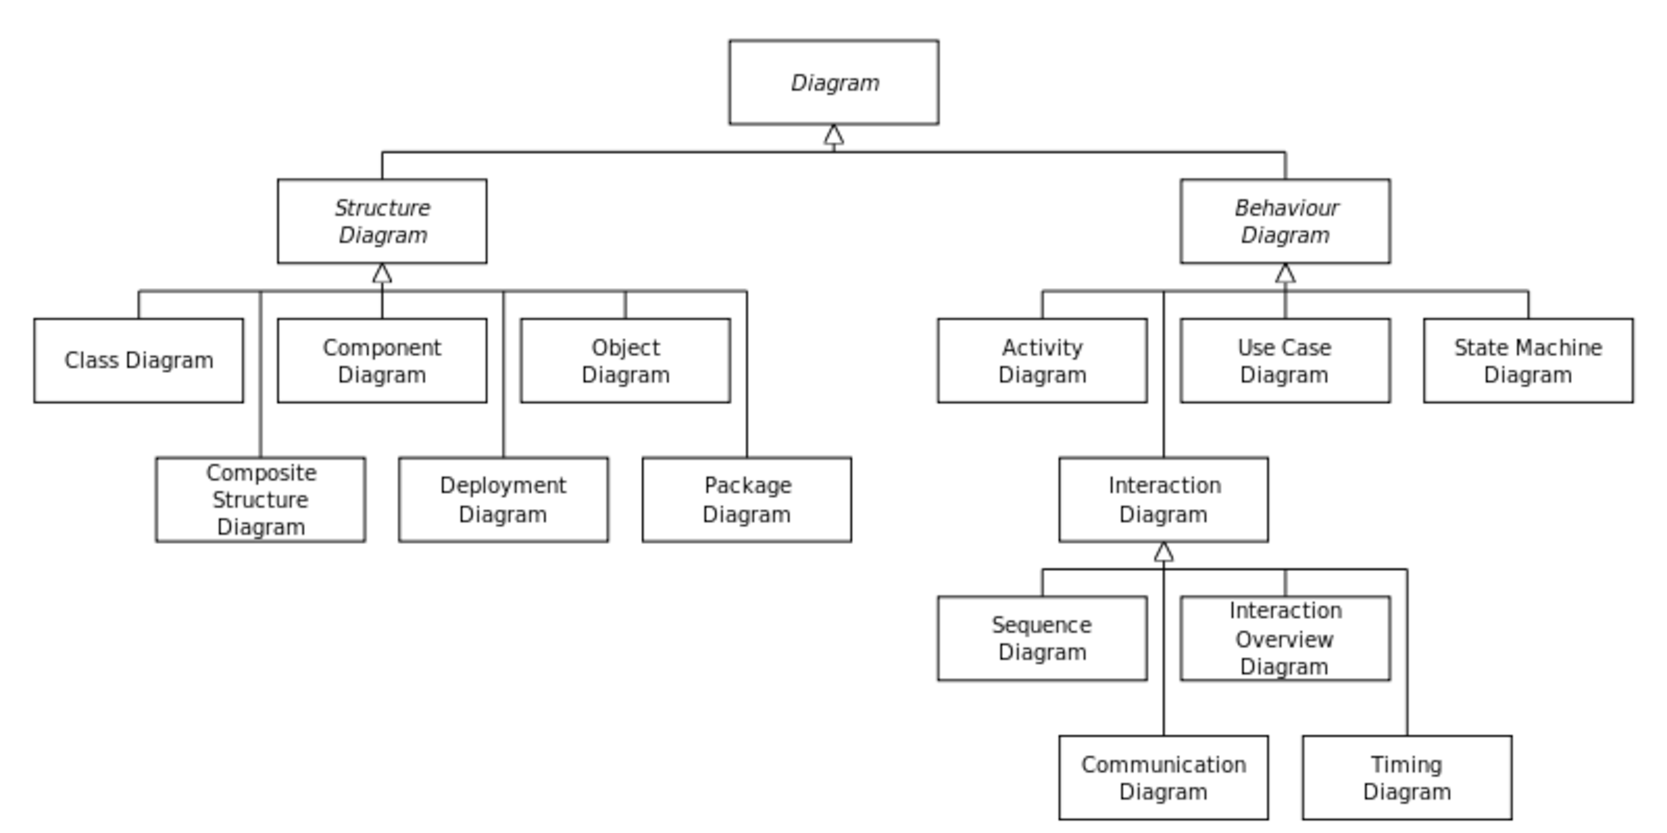
\includegraphics[width=16cm]{exemploFig}
\caption{Exemplo de Figura (\textit{in} \url{http://en.wikipedia.org/wiki/Class_diagram})}
\label{fig:exemplofig}
\end{figure}

Exemplos de citações \cite{AndroidDoc},
\cite{Huetal2000,book:Brooks1995,Chen1976}

%Exemplo de listagem de código Java.
%\lstlisting{

\section{Exemplos de Listagens}

A Listagem \ref{lst:py} apresenta um exemplo de implementação do algoritmo de ordenação \textit{quicksort} na linguagem de programação Python.

\begin{lstlisting}[language=python,caption={Exemplo de listagem de código Pythonescrito directamente no ficehiro tex (apenas recomendado para 1 a 5 linhas de código},{label=lst:py}]
# in http://www.ics.uci.edu/~eppstein/161/python/quicksort-inplace.py - 2013/04/14
# quick sort, in-place 3-way partition
# David Eppstein, UCI, 17 Jan 2002
def swap(A,i,j):
	temp = A[i]
	A[i] = A[j]
	A[j] = temp
\end{lstlisting}


A Listagem \ref{lst:java} apresenta um exemplo de implementação do algoritmo de ordenação \textit{quicksort} na linguagem de programação \Java{}.

\lstinputlisting[language=java,caption={Exemplo de listagem de código Java importado de um ficheiro na pasta listagens.},{label=lst:java}]{listagens/quicksort.java}

\lstinputlisting[language=java,caption={Exemplo de listagem de parte de um ficheiro Java na pasta listagens.},{label=lst:javaparcial},firstline=38,lastline=44]{listagens/quicksort.java}


\pagebreak % para forçar uma mudança de página
%%%%%%%%%%%%%%%%%%%%
\section{Um exemplo de tabela}

A Tabela \ref{tab:caso} apresenta os resultados de aplicação de quatro métodos a um caso.

%baseado num exemplo em http://www1.maths.leeds.ac.uk/latex/TableHelp1.pdf
\begin{table}[htb]
\caption{Uma tabela de exemplo} % título da tabela
\centering % para centrar a tabela
\begin{tabular}{l l c r} % duas colunas à esquerda (l l), uma ao centro (c) e uma à direita (r) (4 colunas)
\hline\hline %insere duas linhas horizontais
Caso & Método 1 & Método 2 & Método 3 \\ [0.5ex] % insere tabela 
\hline % insere uma linha horizontal
1 & 50 & 837 & 970 \\ % insure corpo da tabela
2 & 47 & 877 & 230 \\
3 & 31 & 25 & 415 \\
4 & 35 & 144 & 2356 \\
5 & 45 & 300 & 556 \\ [1ex] % [1ex] adiciona espaço vertical
\hline %insere uma linha horizontal
\end{tabular}
\label{tab:caso} % é utilizada para referir a tabela no texto
\end{table}





\chapter{Título do Capítulo 3}
\label{cap3}

Mais umas citações \cite{AndroidDoc, Chen1976}

%a linha seguinte deve ser substituída pelo texto do capítulo
\lipsum


% para adicionar o  capítulo N adicione a linha \input{capituloN} e crie o ficheiro 
% capituloN.tex na directoria "capitulos" 


%%%%%%%%%%%%%%%%%%%%%%%%%%%%%%%%%%%%%%%%%%%%%%%%
% Bibliografia
\clearpage
\printbibliography[heading=bibintoc]
%%%%%%%%%%%%%%%%%%%%%%%%%%%%%%%%%%%%%%%%%%%%%%%%
\apendices
\chapter{\textit{Jupyter Notebook} da Extração de Palavras-Chave}
\label{ap1}

%a linha seguinte deve ser substituída pelo texto do apêndice

Nas paginas seguintes está incluída uma renderização do \textit{notebook} de \textit{Jupyter} em que se detalha (em inglês) os passos das rotinas de extracção de palavras-chave, comentando de forma simples o funcionamento das funções de código usadas.

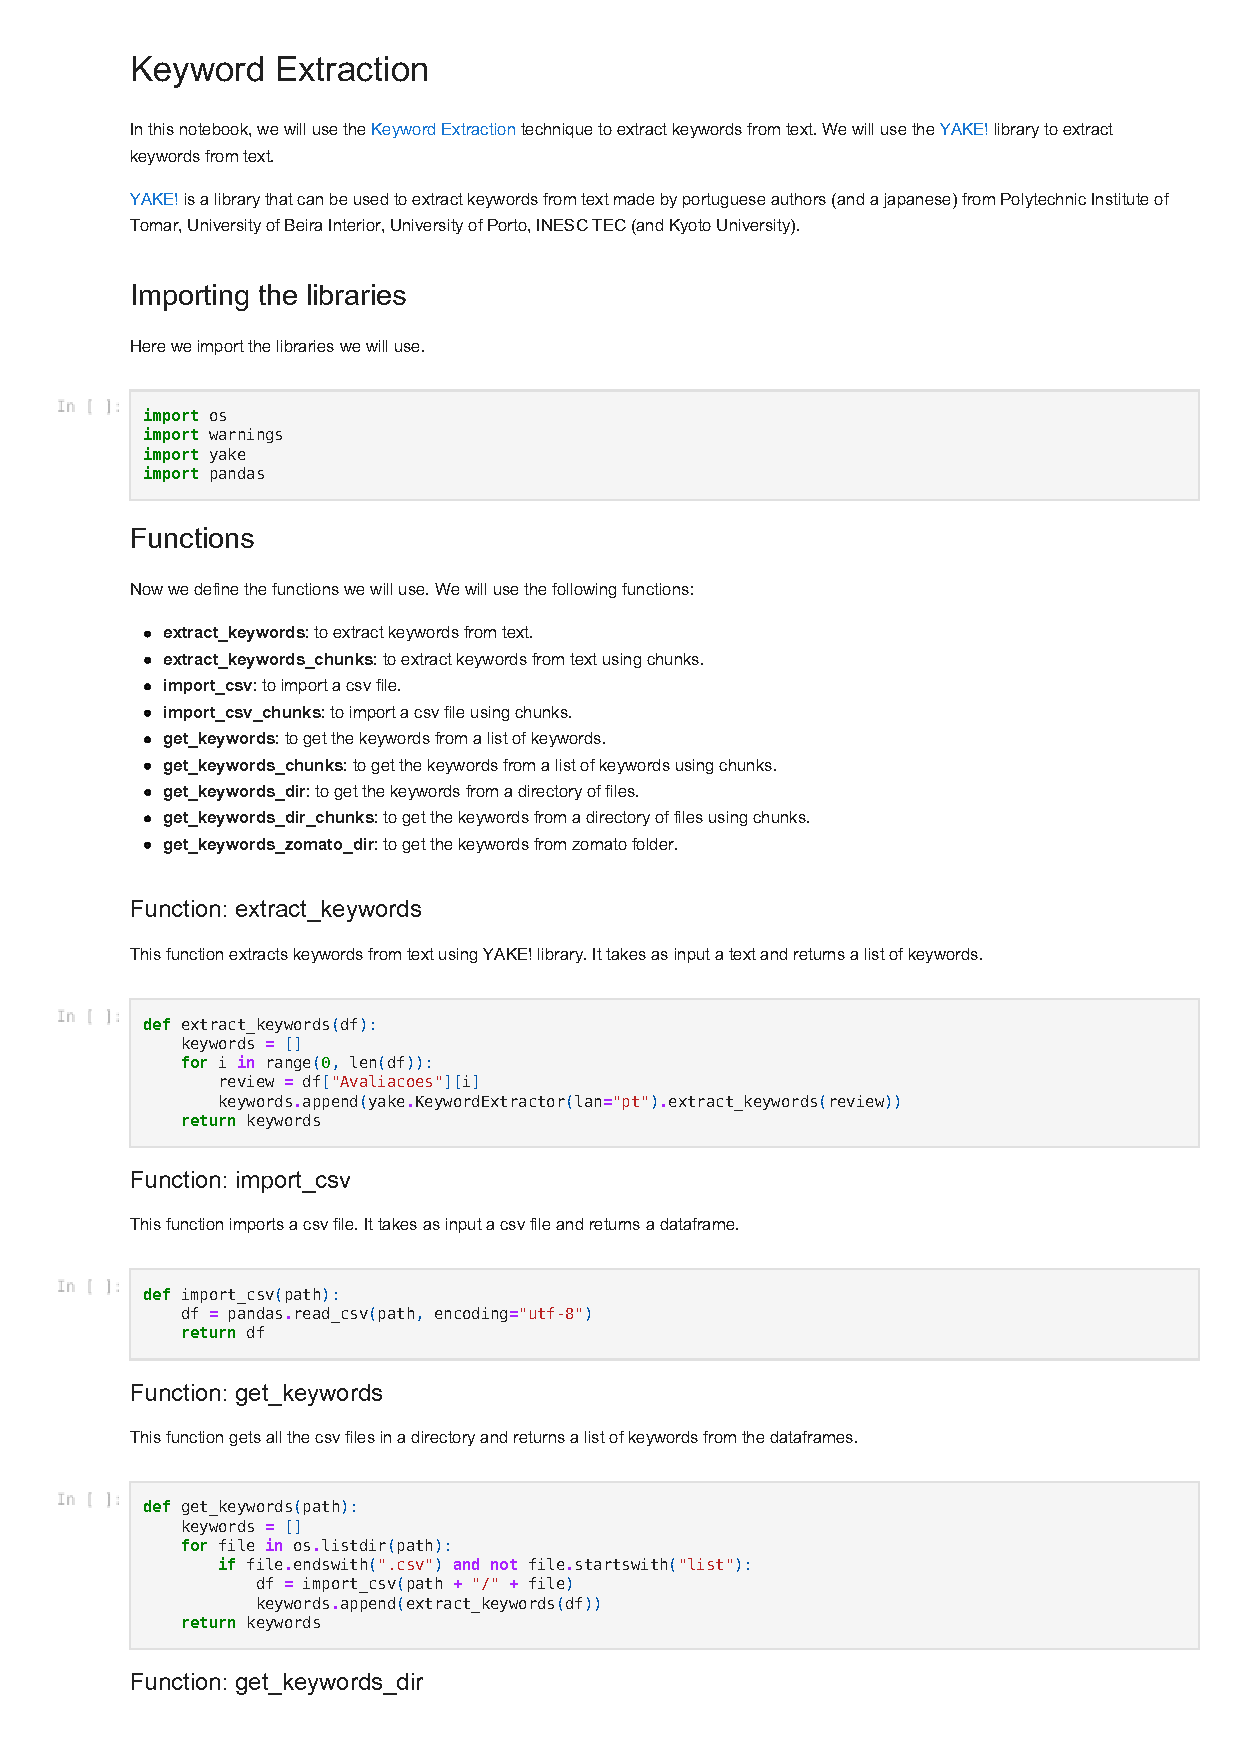
\includepdf[pages=-2,scale=0.75]{jupyter/ta-kwe.pdf}
% para adicionar o  apêndice N adicione a linha \input{apendiceN} e crie o ficheiro 
% apendiceN.tex na directoria "apendices" 
%%%%%%%%%%%%%%%%%%%%%%%%%%%%%%%%%%%%%%%%%%%%%%%%
\anexos
\chapter{Anexo referente às imagens dos gráficos utilizados no relatório (TripAdvisor-Hóteis)}
\label{an1}

Uma vez que as imagens que retratam os gráficos elaborados são muito extensas, serão apenas mostradas algumas delas e em, cada secção apontado o link que redirecciona para o GitHub do projecto onde será possível aceder a cada imagem respectivamente assim como ao ficheiro \textit{.pbix} que contém os gráficos realizados no \textit{PowerBI}.
Inicialmente serão expostos os gráficos totais, anteriormente mostrados no \hyperref[cap7]{ capítulo 7 (Geração de gráficos)} exclusivamente para o \textit{website TripAdvisor} e acerca dos hotéis.

Acesso a todos os gráficos originados: \href{https://github.com/CatKinKitKat/pi2021/tree/master/projecto/datascience/graphs/TripAdvisor/hotels}{GitHub}.

\begin{figure}[!htb]
\centering
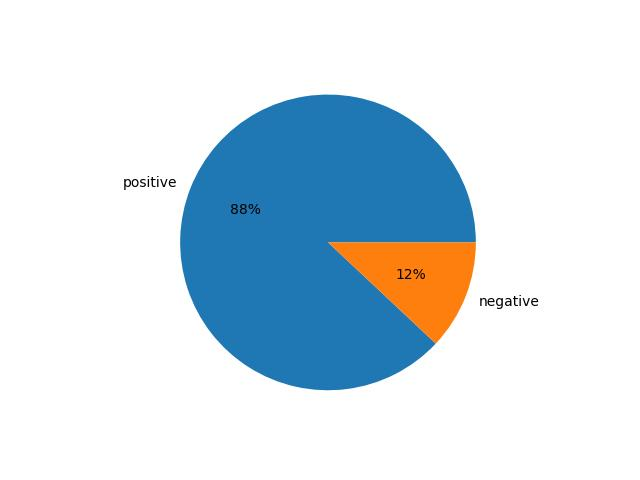
\includegraphics[width=7cm]{figuras/TripAdvisor/Hotels/hotel0_sentiments.jpeg}
\caption{Gráfico circular gerado baseando-se nos \textit{sentiments} mais usados da plataforma \textit{TripAdvisor} referente à Pousada Convento Beja}
\label{fig:exemplofig}
\end{figure}

\begin{figure}[!htb]
\centering
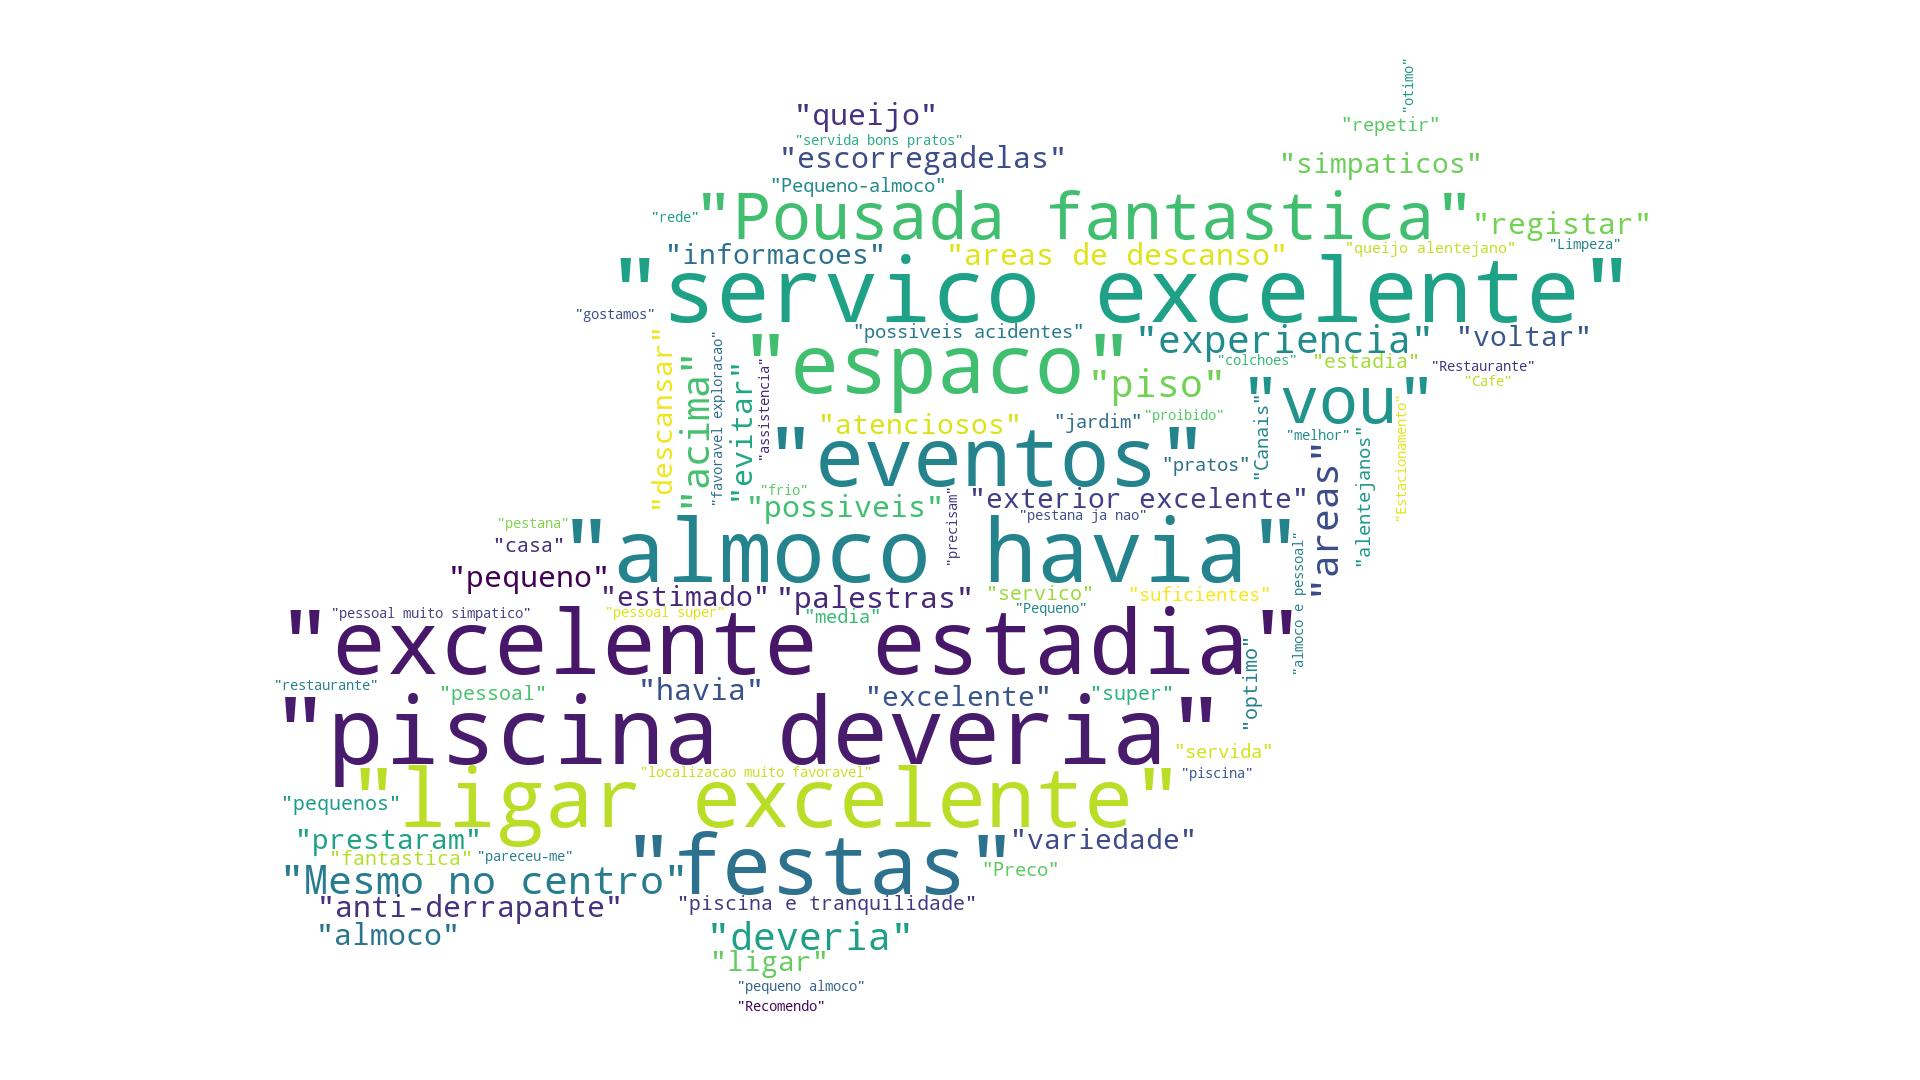
\includegraphics[width=7cm]{figuras/TripAdvisor/Hotels/hotel0_keywordcloud.jpeg}
\caption{Gráfico de palavras-chave e nuvens de palavras-chave contendo as \textit{keywords} mais usadas da plataforma \textit{TripAdvisor} referente à Pousada Convento Beja}
\label{fig:exemplofig}
\end{figure}

\begin{figure}[!htb]
\centering
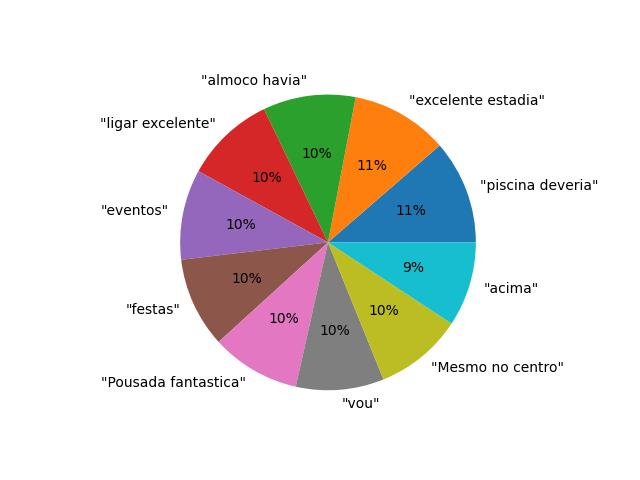
\includegraphics[width=7cm]{figuras/TripAdvisor/Hotels/hotel0_keywords.jpeg}
\caption{Gráfico circular gerado baseando-se nas \textit{keywords} mais usadas da plataforma \textit{TripAdvisor} referente à Pousada Convento Beja}
\label{fig:exemplofig}
\end{figure}

\begin{figure}[!htb]
\centering
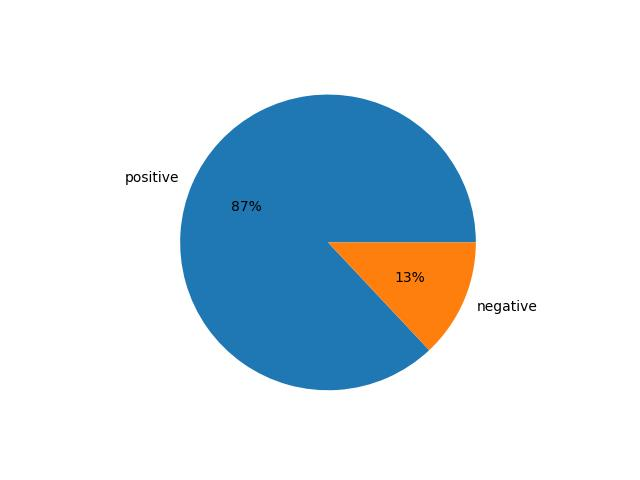
\includegraphics[width=7cm]{figuras/TripAdvisor/Hotels/hotel8_sentiments.jpeg}
\caption{Gráfico circular gerado baseando-se nos \textit{sentiments} mais usados da plataforma \textit{TripAdvisor} referente ao Hotel São Domingos}
\label{fig:exemplofig}
\end{figure}

\begin{figure}[!htb]
\centering
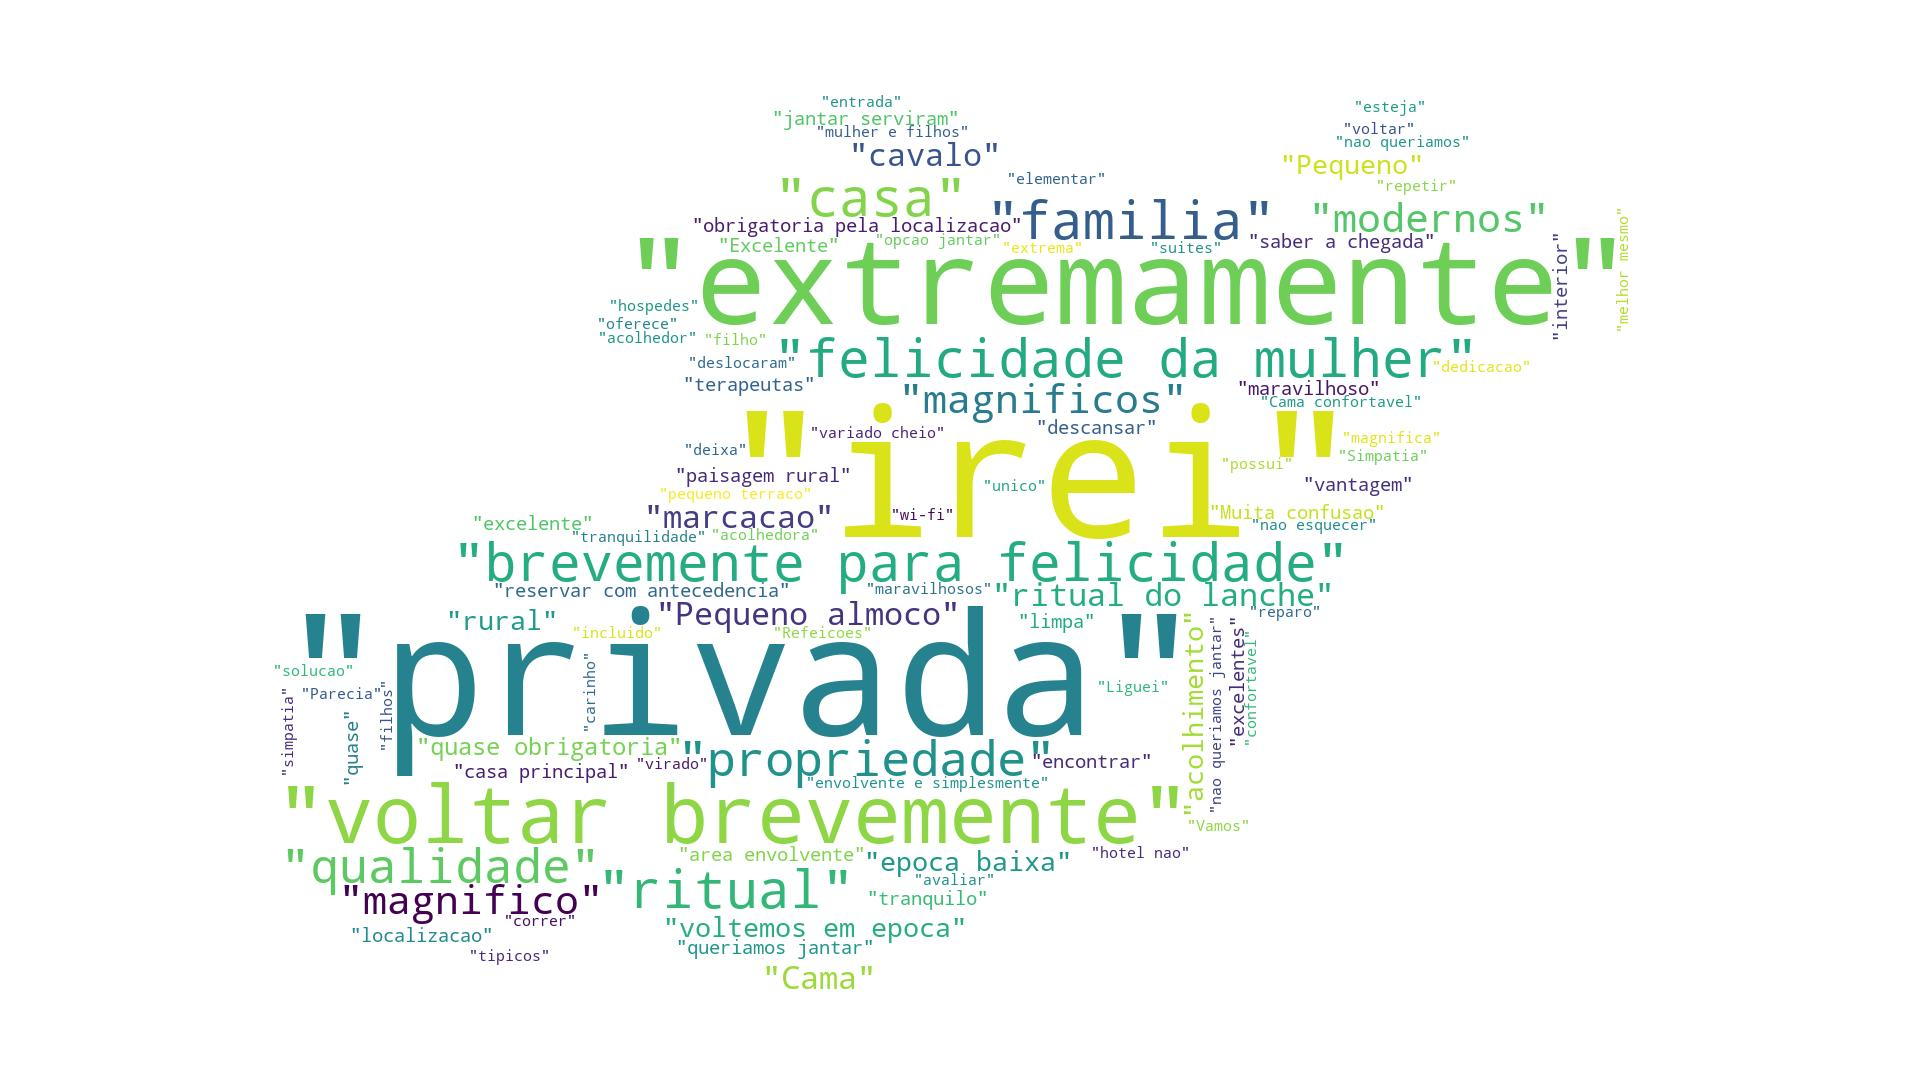
\includegraphics[width=7cm]{figuras/TripAdvisor/Hotels/hotel8_keywordcloud.jpeg}
\caption{Gráfico de palavras-chave e nuvens de palavras-chave contendo as \textit{keywords} mais usadas da plataforma \textit{TripAdvisor} referente ao Hotel São Domingos}
\label{fig:exemplofig}
\end{figure}

\begin{figure}[!htb]
\centering
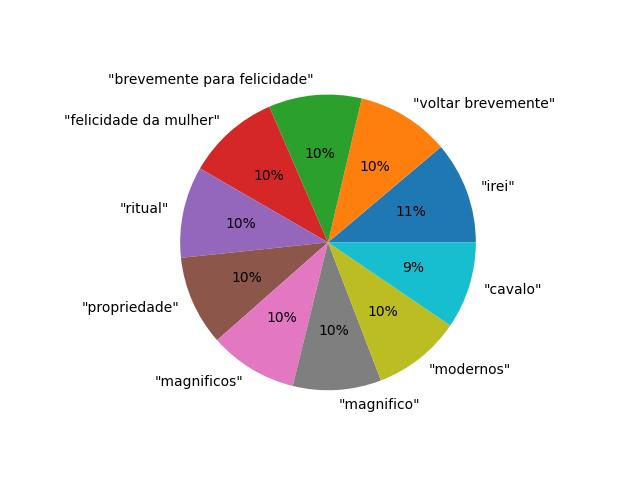
\includegraphics[width=7cm]{figuras/TripAdvisor/Hotels/hotel8_keywords.jpeg}
\caption{Gráfico circular gerado baseando-se nas \textit{keywords} mais usadas da plataforma \textit{TripAdvisor} referente ao Hotel São Domingos}
\label{fig:exemplofig}
\end{figure}

\begin{figure}[!htb]
\centering
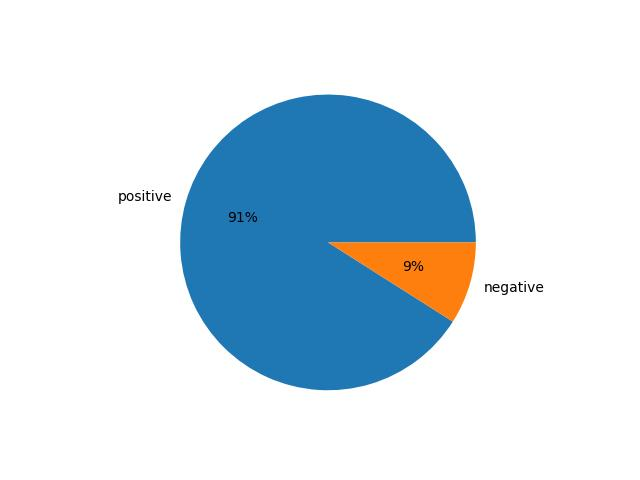
\includegraphics[width=7cm]{figuras/TripAdvisor/Hotels/hotel21_sentiments.jpeg}
\caption{Gráfico circular gerado baseando-se nos \textit{sentiments} mais usados da plataforma \textit{TripAdvisor} referente à Herdade das Barradas da Serra}
\label{fig:exemplofig}
\end{figure}

\begin{figure}[!htb]
\centering
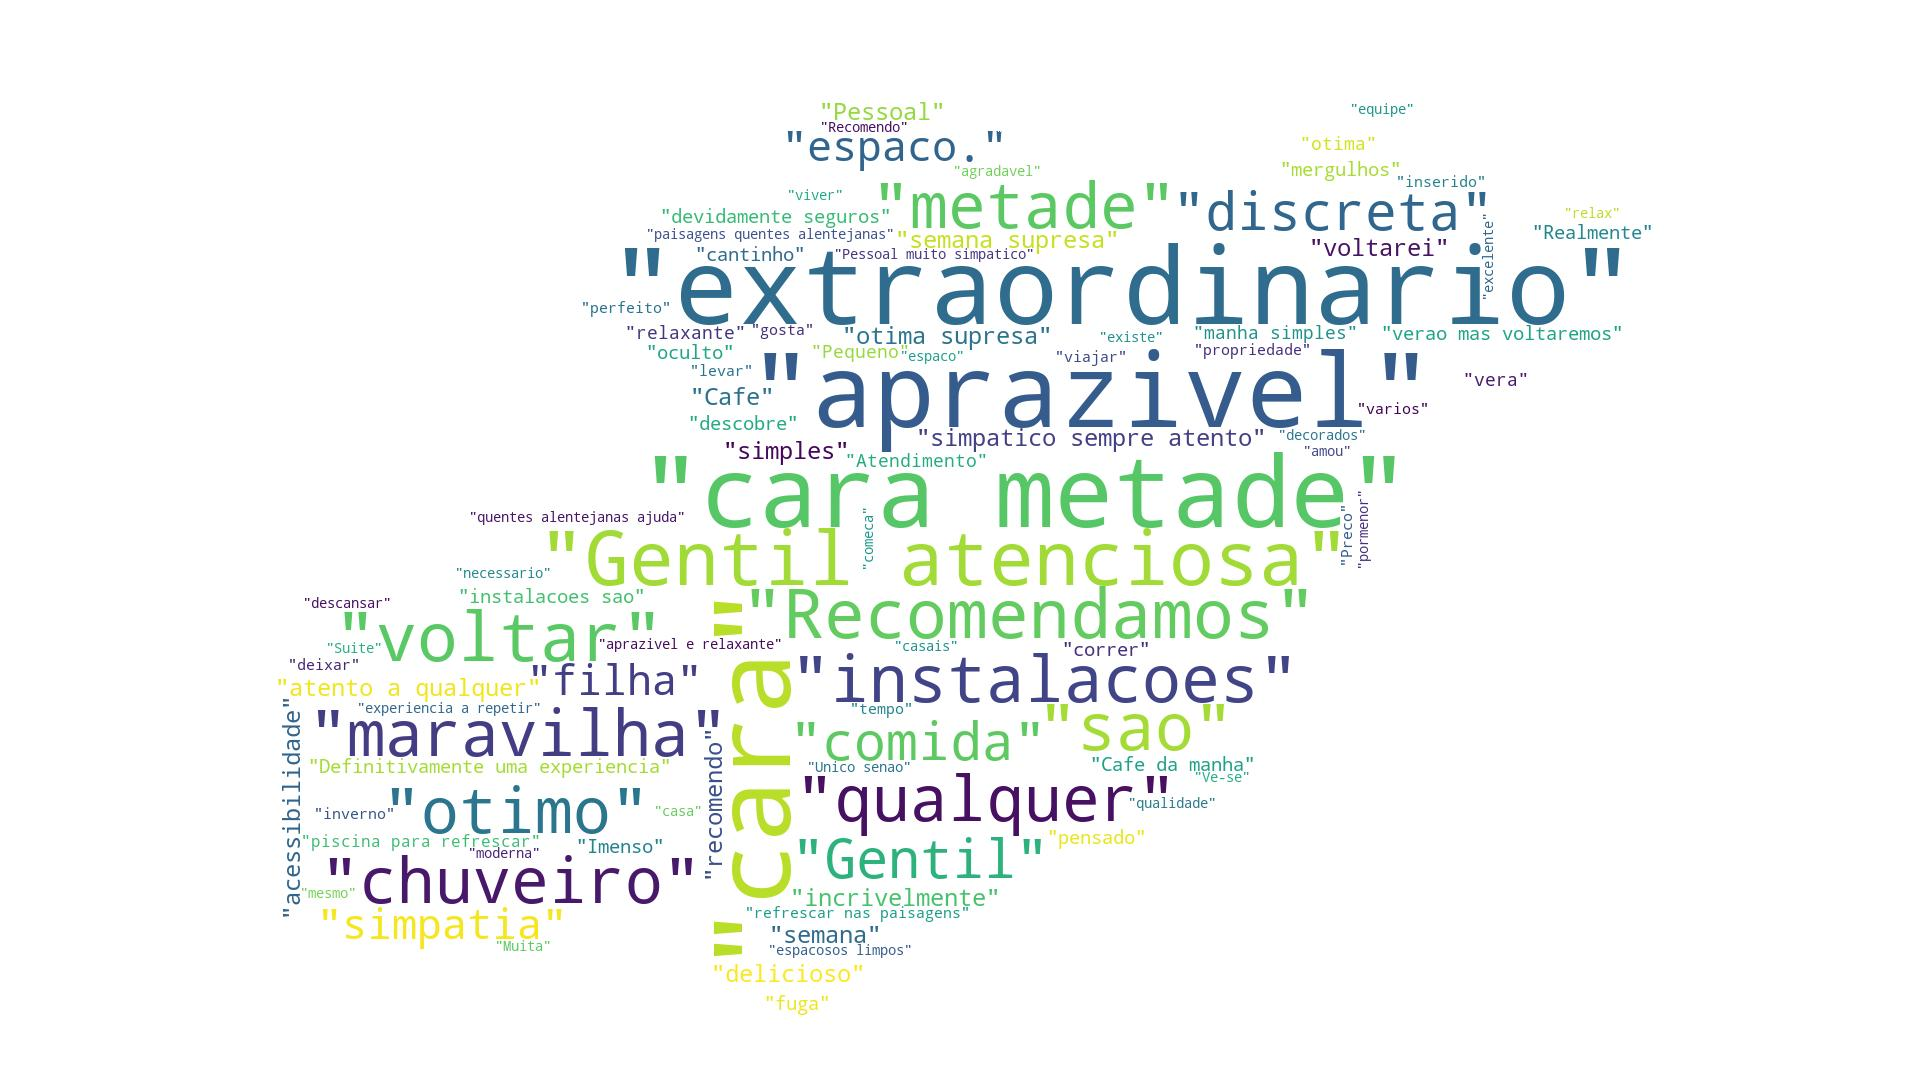
\includegraphics[width=7cm]{figuras/TripAdvisor/Hotels/hotel21_keywordcloud.jpeg}
\caption{Gráfico de palavras-chave e nuvens de palavras-chave contendo as \textit{keywords} mais usadas da plataforma \textit{TripAdvisor} referente à Herdade das Barradas da Serra}
\label{fig:exemplofig}
\end{figure}

\begin{figure}[!htb]
\centering
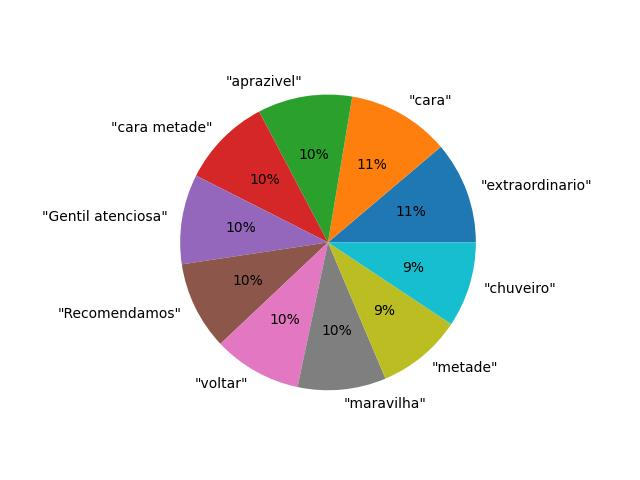
\includegraphics[width=7cm]{figuras/TripAdvisor/Hotels/hotel21_keywords.jpeg}
\caption{Gráfico circular gerado baseando-se nas \textit{keywords} mais usadas da plataforma \textit{TripAdvisor} referente à Herdade das Barradas da Serra}
\label{fig:exemplofig}
\end{figure}


% para adicionar o  anexo N adicione a linha \input{anexoN} e crie o ficheiro 
% anexoN.tex na directoria "anexos" 
%%%%%%%%%%%%%%%%%%%%%%%%%%%%%%%%%%%%%%%%%%%%%%%%


\vfill
{\footnotesize Documento elaborado com base no \ing{template for final reports and dissertations (Instituto Politécnico de Beja)}, disponível em \url{https://www.overleaf.com/project/5d936b9ea273390001434a37}, Version 0.8.1, 2021/10/01, Author: João Paulo Barros, joao.barros@ipbeja.pt}
\end{document}